\documentclass[times, utf8, diplomski]{fer}
\usepackage{booktabs}
\usepackage{pdfpages}
\usepackage{catchfile}
\usepackage{xparse}
\usepackage{listings}
\usepackage{nameref}
\usepackage{float}


\renewcommand{\labelitemi}{$\bullet$}

\usepackage{amsthm}
\theoremstyle{definition}
\newtheorem{definition}{Definition}[]

% environment setup
\ExplSyntaxOn
\NewDocumentCommand{\getenv}{om}
 {
  \sys_get_shell:nnN { kpsewhich ~ --var-value ~ #2 } { } \l_tmpa_tl
  \tl_trim_spaces:N \l_tmpa_tl
  \IfNoValueTF { #1 }
   {
    \tl_use:N \l_tmpa_tl
   }
   {
    \tl_set_eq:NN #1 \l_tmpa_tl
   }
 }
\ExplSyntaxOff

\getenv[\resdir]{THESIS_RESDIR}
% done

\newcommand{\pythoncode}[3]{
    \lstinputlisting[xleftmargin=20pt, basicstyle=\small, numbers=left, 
    label=#2, caption=#3, language=Python]{#1}
}

\newcommand{\agtcode}[3]{
    \lstinputlisting[xleftmargin=20pt, basicstyle=\small, numbers=left, 
    label=#2, caption=#3, morekeywords={
        if, else, break, for, while, return,
        fn, struct, let, type,
    }]{#1}
}

\newcommand{\textcode}[3]{
    \lstinputlisting[xleftmargin=20pt, basicstyle=\small, numbers=left, 
    label=#2, caption=#3,
    ]{#1}
}

\begin{document}
\sloppy
\thesisnumber{2568}

\title{Design of a strongly-typed programming language}

\author{Petar Mihalj}

\maketitle

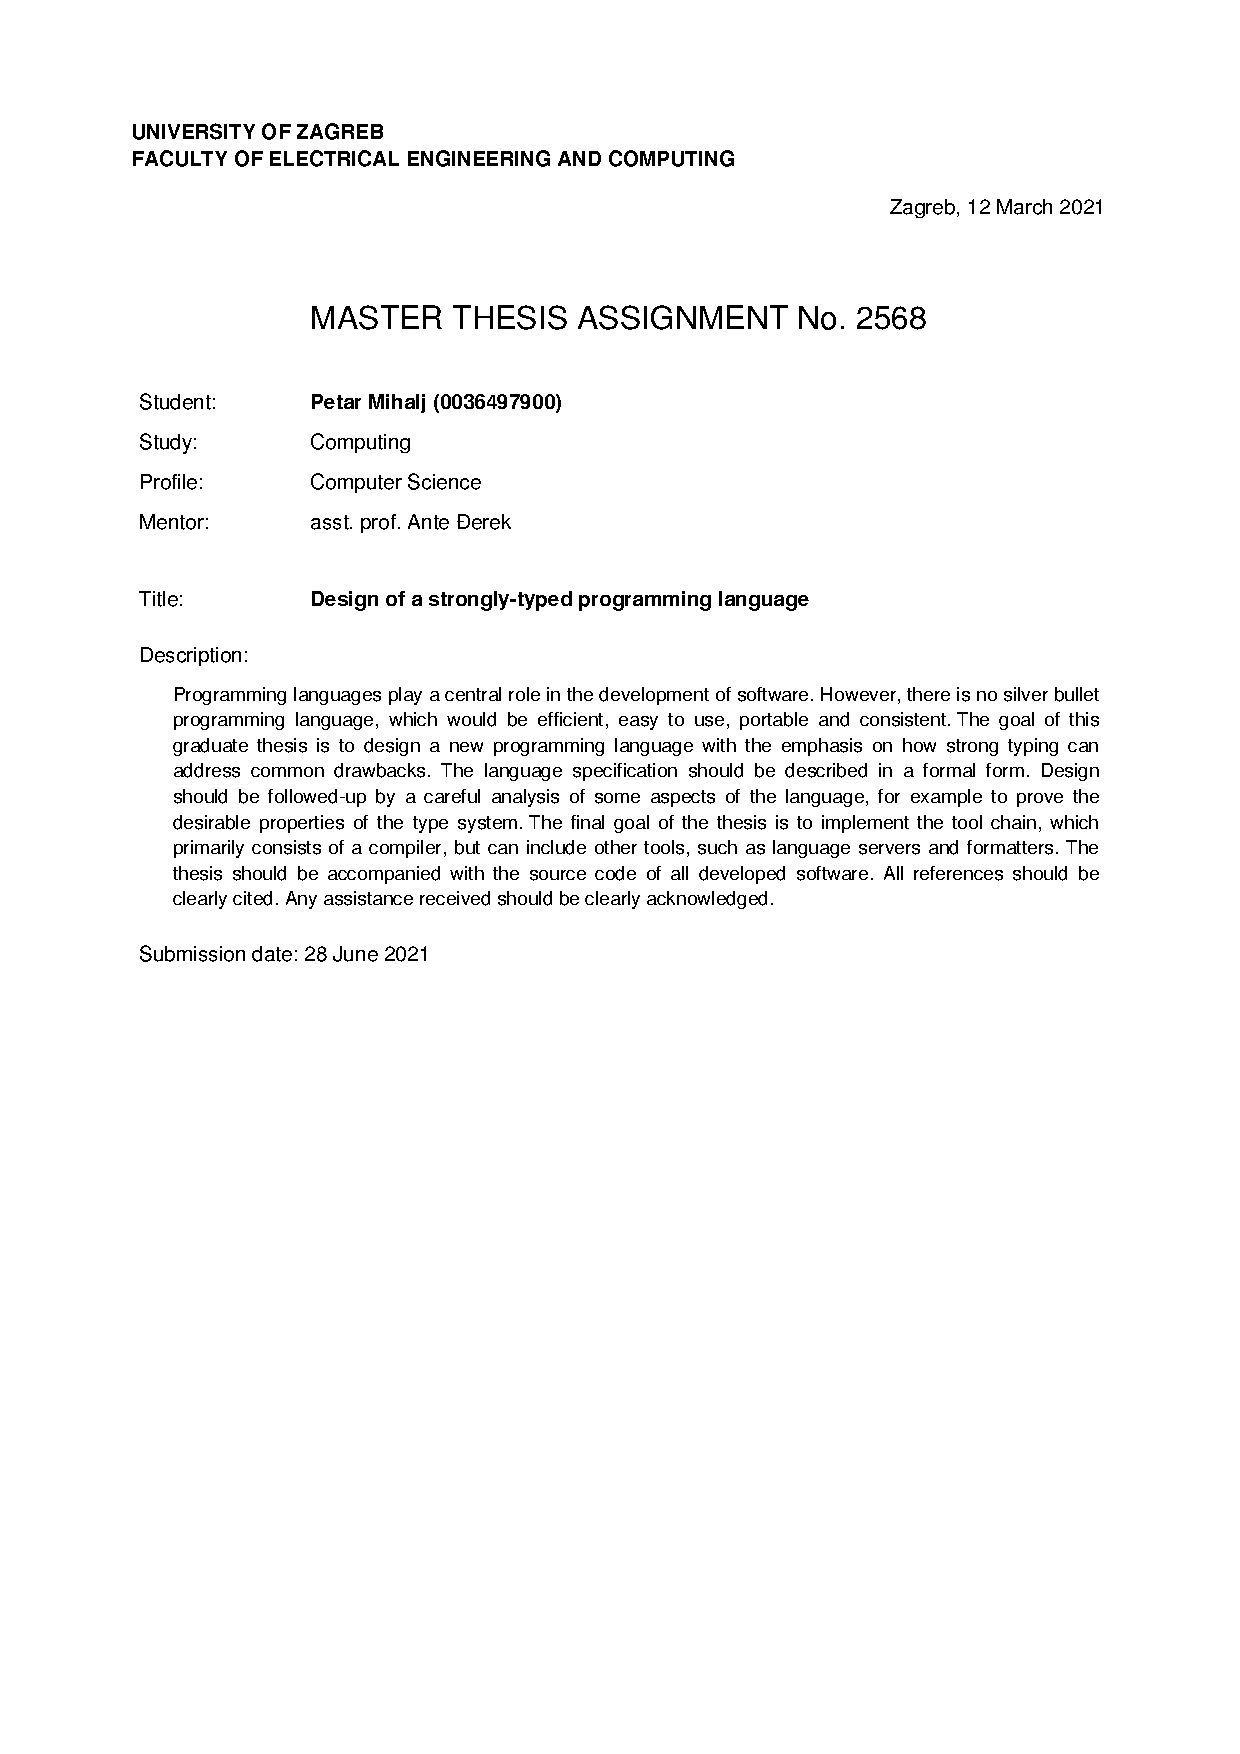
\includepdf[pages={1,2}]{\resdir/task.pdf}

\zahvala{I thank everybody...}

\tableofcontents

\chapter{Introduction}\label{chap:intro}

The programming language developed as a part of this thesis is called AGT.
The name AGT stands for an unfortunate fact that the names of all precious stones
are taken by other programming languages, hence "All Gems are Taken".

\textbf{The AGT programming language} is a statically \citep{c_static_typing} and 
strongly \citep{c_strong_typing} typed language, with a highly expressive type system.
The type system is used for three main purposes:

\begin{enumerate}
    \item types determine the memory footprint of values 
    \item types allow for polymorphic behaviour of operators and functions on all 
        \textit{concrete types} (built-in or struct types)
    \item type system lets the programmer perform compile-time computation
\end{enumerate}

The language also allows for implementation of object lifetime constructs, 
such as those seen in languages such as C++ \citep{c_cpp_lifetime}; 
object creation, copying and destruction.

\textbf{The reference AGT compiler (AGTC)} produces executable binaries only.
This is in sharp contrast to some other languages, which can produce object files, 
to later be linked into executables for a particular runtime, 
or used to augment the runtime environment itself (kernel modules, for example). 
This decision was made primarily because the goal of the thesis was to study the language 
from the application programmer's perspective. 
This goal requires that AGT is running on a rich runtime environment, 
where heap memory management and standard I/O are available.
Future updates to AGT specification are meant to allow AGT to be compiled
into linkable files compatible with various platform specific ABIs.

The compiler frontend is implemented using Python3 programming language version 3.9.5 (but should work
on all versions starting from 3.7),
while the backend uses LLVM compiler infrastructure \citep{c_llvm_lattner}.
Allowing for some simplification, AGT is first compiled into LLVM intermediate representation (LLVM-IR),
and than is turned into executable by a chain of tools for compiling LLVM-IR and 
linking the resulting object files into executables.

\section{Example program}

Let us first check out an example AGT program in listing \ref{intro.agt}:

\agtcode{\resdir/programs/intro.agt}{intro.agt}{Example AGT program}

Every AGT program has to have a function definition named \texttt{main}, 
which returns a 32-bit-wide integer,
and has no parameters.
Some functions, like \texttt{outnl}, don't return anything. 
There is no \texttt{void} type for functions that don't return a value;
just skip specifying the return type to achieve this behaviour.

A \texttt{let <x> = <y>;} construct is an \textit{initialization assignment statement}.
This roughly translates to an allocation of memory on the stack (which can be referred
to as the \textit{location} of <x> from now on), and copying the value of expression <y>
to the location of identifier <x>.

Note that the function call \texttt{in} (line 11) is \textit{parametrized} 
by a \textit{type argument} \texttt{i32}.
Type arguments are used to pass types, but not values, to functions. 
They are different than \textit{value arguments}, which carry value too, along with a type.
The \textit{passing} of type parameters is purely a compile-time concept;
types can't be referred to during runtime.


The function \texttt{in} is a built-in, and the \texttt{i32} is used to signal the compiler
that we want an instance of this function which returns an \texttt{i32}, 
instead of a \texttt{bool}, for example. 
Of course, user-defined functions can also have \textit{type parameters}, along with \textit{value parameters};
we will get to these later.

Notice that we used the \texttt{cast<i32>} built-in function to convert \texttt{b} to \texttt{i32}
before passing it to function \texttt{mul}. If we didn't do that, the compiler would signal that it can't
compute the expression \texttt{a*b}, since multiplication is predefined only for integer types of same size.
Apart from the \texttt{i8} and \texttt{i32} we used in this example, \texttt{i16} and \texttt{i64} are also
available.

Also, notice that line 6 is terminated by \texttt{-> a}. This is a \textit{return type specification};
it states that this function will return a value with a type being equal to whatever is type of \texttt{a}. 

You might have noticed a certain feature while inspecting the code; 
namely the absence of explicitly stated types in the signature of function definition \texttt{mul}.
While some \textit{dynamically typed} languages (for example Python) allow for object of any type to be passed
to the function, AGT behaves quite differently. 

Every time AGTC (AGT compiler) encounters a function call,
it tries to infer a \textit{function type}. Function type is inferred either from user-supplied function 
definitions, or from built-in function type generators (more on the this later).
Consequently, you can think of the definitions in source code as \textit{templates} for synthesis
of actual code. In other words, for each function definition there might be more than one
function type inferred from it.

These definitions lack types, and can't be considered in isolation.
In this example, it is the call of function \texttt{mul} which causes
the compiler to try to infer a function type.
Parameters of \texttt{mul} function definition (\texttt{a, b}) can be fit with objects of
any type; it is after this fitting that the compiler will determine that passed types can or can't
be used (due to their incompatibility with a function definition body, for example).

It is important to emphasize that one function definition can be a source of many function types.
The \texttt{outnl} (output with newline) function is a prime example of this behaviour.
It is called three times, with argument of types \texttt{i32}, \texttt{i8} and \texttt{i32}.
Thus, the compiler has to infer two function types, 
one which can be fed with an \texttt{i8}, and one with \texttt{i32}.
The success of this inference is mainly to do with compilers ability to infer functionality of 
body of the given function definition.

In this case, inference of function definition body will be possible if both function calls on lines
2 and 3 can be inferred. Since \texttt{out} function is a built-in for both \textt{i32} and \textt{i8},
line 2 won't be problematic for inference. Line 3 will be inferred correctly if AGTC succeeds to resolve
function type \texttt{out} which takes in a value argument of type \texttt{char}. 
Since this \textit{version} of \texttt{out} also a built-in,
inference of function types for both versions of \texttt{mul} succeeds.

The property of AGT \textbf{function calls} which can make them refer to different function types, 
when called with different sets of arguments, is called \textit{polymorphism} \citep{c_polymorphism}.
Some sources label polymorphic the very \textbf{function definitions} which, when called upon, 
can result in such behaviour.
We will use these conventions interchangeably, since the definition itself is non-rigorous.

Function definition of \texttt{outnl} introduces a special type of polymorphism, 
\textit{parametric polymorphism}. This polymorphic behaviour is said to be present if the
function definition can be a source for potentially unlimited number of types, 
as long as those types are compatible with function definition body.

Python programming language exhibits a superficially similar behaviour, but its
function body compatibility checks occur at runtime. 
The programming style which utilizes this language capability is often called "Duck Typing" 
\citep{c_py_duck_typing} in dynamically typed languages.


\section{Paper organization}

This master thesis will gradually introduce the reader to AGT. 

Chapter \ref{chap:intro} has already introduced the reader to basic syntax and semantics,
using a simple example and emphasizing the surface-level properties of type system and inference. 

The following chapter \ref{chap:design} will lay out and justify author's
language design decisions. The discussion includes many diverse topics,
ranging from syntactical decisions, to subtle semantic onces.

After the surface-level exploration of the language, chapter \ref{chap:indepth}
will provide an in-depth description of AGT.
This chapter will have many references to the AGTC reference implementation, 
rather than to a separate formal specification. Since AGT is still not a finalized product,
formal specification does not exist, and it's functionality is determined by a reference compiler.
We will mostly focus on the type system, since it is unorthodox and is the main
contribution of the author.  Author will justify the decisions which had been
made on all levels of AGT design process.

Chapter \ref{chap:examples} will supplement the reader with plenty of examples of AGT code. These will
further deepen reader's understanding of AGT. The examples describe implementation
of common programming paradigms, constructs and patterns in AGT, with a detailed
explanation of more esoteric parts of the source code.

In chapter \ref{chap:improv} we will address the issues AGT has both on
definition and implementation levels, and discuss the various features that can
be improved upon or added to the language.

Chapter \ref{chap:concl} will conclude the thesis and describe future work the
author will undertake in order to improve the language.

\chapter{Design decisions}\label{chap:design}

In this chapter we will describe and justify the main design decisions concerning AGT,
weighing their positive and negative sides against one another.

\section{Syntax}

Main inspiration for AGT's syntax have been well-known languages C and C++.
Since most programmers are familiar with these, it is only logical not to diverge from their syntax,
whenever possible.
Of course, AGT is way more implicit in typing than both C and C++, that is, types have to be specified
only when necessary (for example, when limiting function polymorphism according to types).
Implicit typing allows the programmer to focus on logic instead of specifying redundant type annotations
(such as in C), or keywords that signal the compiler to perform automatic type
inference, such as \texttt{auto} in C++ \citep{c_auto}.

On the other hand, the absence of explicit type specification can make the program more unreadable,
due to the lack of hints these types provide. 

The author would argue that such problems are
rooted in more subtle problems, such as poorly designed function interfaces.
If the function definition is named \texttt{square}, 
it is only natural to assume that a supplied argument can be multiplied by itself.
Function definitions that are more convoluted than \texttt{square} can explicitly state their requirements
in the beginning of function definition body, thus giving the programmer a hint for their usage. 

The Rust Programming Language has had a significant impact on AGT's syntactical features too.
Mainly, it's use of clear function definition syntax and \texttt{let} statement syntax is
embedded deeply into AGT.

The Zen of Python \citep{c_zen} is a set of guidelines for writing clean, \textit{pythonic} code. 
One of these guidelines - \textit{Explicit is better than implicit}, has had a huge impact on AGT.
Starting from clean function definition syntax, to explicitly named operator (\textit{dunder}) functions
(\texttt{\_\_add\_\_, \_\_init\_\_, ...}), AGT places explicitness over surface-level practicality.
The author would argue that explicit code is more readable, maintainable and safe over long term,
which is a big win over a small expense of writing a few more characters.
Object creation is also as explicit as can be, whether on the stack or the heap.

Another guideline from The Zen of Python is 
\textit{There should be one and preferably only one obvious way to do it}. 
AGT tries to inhibit programmer's choice in a fundamentally non-limiting way, for example, by
having only one syntax for initializing objects. This does not decrease the 
language's expressiveness, but helps avoid confusion and errors.

\section{Type System}

Before going into decisions regarding the AGT type system, we will first state a common
definition of what \texit{type system} actually is, and what we refer to when discussing it.
There are many definitions of type system, 
but the one which captures the essence most precisely is the following:

\textit{A type system is a logical system comprising a set of rules that 
    assigns a property called a type to the various constructs of a computer program, 
such as variables, expressions, functions or modules ... }\citep{c_type_system}.

AGT's type system serves multiple purposes. One is to allow compile time computation.
The most important purpose is to ensure the correctness of programs, both on compile time and run time.

AGT's type system is \textit{static} \citep{c_static_typing}, that is, 
all values have types which can be, and are, determined
at compile time. Furthermore, all polymorphic behaviour is resolved in compile time, unlike in C++,
where the programmer can use \textit{dynamic dispatch and polymorphism} \citep{c_dyn_dispatch} 
- a run-time dynamic lookup of functions.
This makes AGT even more type-safe, by preventing common mistakes which happen when utilizing
dynamic polymorphism. The author argues that object oriented principles which heavily rely on
dynamic polymorphism (such as inheritance), can mostly be eliminated by better program design.

Another feature of AGT is that it is \textit{strongly typed} \citep{c_strong_typing}. 
Most definitions consider
a language to be strongly typed if it rarely or never implicitly converts
types, which leads to more compile-time errors, but at the same time provides
more safety. AGT never converts types implicitly,
which can, to someone coming from languages such as C, appear tiresome to deal with. On the other hand,
explicitly stating type conversions will have greater benefits for the
programmer in the long run.

Type inference engine which supports AGT's type system can appear difficult to
get used to, but in fact is, at least on the theoretical level, rather simple.
There are no complex inference rules;
every time an inference has to be done, all the inputs required to perform the process must be available.
For example, function's return type is inferred from the return type expression. 
This type expression is evaluated
just before the first runtime statement in function definition body, which
ensures that the function's return type is known in case the function is
recursive (directly or not).

AGT's main polymorphism driver, \texttt{enable\_if}, is motivated by a similar C++ construct
\citep{c_enable_if}. This construct is, unlike in C++, integral driver of type system,
rather than a clever trick to remove functions from overload resolution.

\section{Memory management}

AGT aims to be as fast as possible, which rules out having a dedicated \textit{garbage collector},
present in languages such as Java and Python. AGT's storage is split into two main parts,
stack allocated and heap allocated storage. 

The stack storage is used to support function
execution, and is managed implicitly - allocated on function call, deallocated on function ending.
While this storage type is highly efficient, it prevents the use of a number of programming patterns.
To remedy this situation, languages such as C use heap storage. 

Heap storage is an on-demand storage. Having this storage can allow the programmer to define
objects which outlive the functions they are defined in, using pointers as references to this storage,
rather than implicitly referring to storage location through the use of names.
While heap storage allows for many useful design patterns, it can bring many difficult-to-diagnose
problems to the table, namely:

\begin{itemize}
    \item Memory leaks - programmer forgets to free unused memory
    \item Double free - programmer frees unused memory multiple times
    \item Dangling pointers - programmer uses a pointer which refers to already freed memory
\end{itemize}

These problems have been a major source of headache for programmers over the years and can't be solved
without certain effort on programmer's part. A typical attempt to remedy these is the use of 
smart pointers in languages such as C++. We will explore and implement this approach in 
chapter \ref{chap:examples}.

\section{Compiler implementation}

The reader should be aware that AGT is not yet a complete project, but rather an experiment, 
a work in progress. This state of affairs had author decide to use Python3 as a compiler implementation
language. Rapid prototyping features of Python, along with numerous easy-to-use and available libraries
make it a sound choice for the implementation language. Since Python is slow compared to compiled
languages, a reasonable direction to go in, after AGT matures, would be to switch from Python
to one of the compiled languages, such as C++.

\chapter{The AGT Programming Language}\label{chap:indepth}

AGT compilation process consists of 4 main phases: 

\begin{enumerate}
\item Lexical analysis - tokenization of input source code text
\item Syntactical analysis - rule-based grouping of tokens into an \textit{abstract syntax tree}
\item Semantical analysis - transformation of the syntax tree into a \textit{semantical tree}
\item Code generation - inference of the \texttt{main} function type, and code generation
\end{enumerate}

The process is successful if all the steps succeed.

In this chapter we will describe each phase in great detail, contrasting the
newly defined terms against their use in other languages.

\section{Lexical analysis}

The AGT lexical analysis phase is a standard regular expression parsing process.
Lexical analyzer is fed a stream of characters, which get grouped into tokens,
according to regular expressions and ambiguity resolution rules.

Lexical analyzer tool used for the AGTC is PLY - Python Lex-Yacc \citep{c_ply_beazley}.
Python Lex-Yacc is a tool which attempts to port the functionality of well know
lexical and syntactical analyzers Lex and Yacc into Python. The main difference
is that PLY does not \textit{generate} the 
concrete lexer and parser. Instead, the PLY user defines the rules fed to PLY by
specifying programming 
constructs (functions, for example) that correspond to these rules. 
PLY then inspects these constructs using 
reflective capabilities of Python, and acts according to these rules
when performing lexical or syntactical analysis.

Let us check out the main lexing module of AGTC in listing \ref{lexer}, 
which specifies rules, states and precedence that
PLY uses to perform lexical analysis for AGT. Some parts of the lexing module
are left out, which is indicated by \texttt{\#...} in source code.

\pythoncode{\resdir/compiler/lexer.py}{lexer}{Lexing module}

This lexer module has 3 states: \texttt{main} (implicit), \texttt{mlc} (for multi-line comments) 
and \texttt{strchar} (for \textit{char array literals} or \textt{char} literals).

Rules for simple operators are given in a string form, 
in a form of \texttt{t\_<TOKEN> = <REGEX>}.

Rules for tokens which are defined with more complex regular expressions, 
like integer literals or identifiers, are defined using functions. 
Those functions can also alter the behaviour of the
lexer when such a token is parsed. For example, whenever an identifier is parsed,
the function \texttt{t\_ID} looks up whether the identifier is in a list of reserved
words, and if it is, changes the token's type. This neat trick greatly simplifies
regular expressions, and is taken from official PLY documentation \citep{c_ply_docs_beazley}.

PLY documentation states that priority is given to regular expressions defined by functions, 
in the order in which they are given.
After function-based rule definitions, 
priority is given to string defined rules (the ones with greater regular expression length first).

We employ the \textit{state} feature of PLY lexing module, 
which allows us to change the lexer's behaviour
when it encounters, for example, a beginning of a multi-line comment. 
In that particular case, lexer goes into \texttt{mlc} state.
When in \texttt{mlc} state, lexer parses and caches every 
symbol until it gets to the end of the comment. 
Both types of comments, \texttt{/*multi-line comment*/} and \texttt{//single-line comment} are discarded
after being parsed.

\subsection{Literals}

Char array literals and char literals are given in double and single quotes, respectively.
They can include escaped characters:  (\textbackslash 0, \textbackslash n, \textbackslash t, 
\textbackslash ", \textbackslash \textquotesingle). 
Character literal must consist of exactly one character or escaped character.

Integer literals are characterized by both the value and the size of integer containing this value.
Possible integer sizes are 8, 16, 32 and 64.

Example integer literals are:
\begin{itemize}
    \item \texttt{5} (implicitly \texttt{i32})
    \item \texttt{5i32}
    \item \texttt{516}
    \item \texttt{5i8}
    \item \texttt{5i64}
    \item \texttt{324243} (implicitly \texttt{i32})
\end{itemize}

Boolean literals are:

\begin{itemize}
    \item \texttt{true}
    \item \texttt{True}
    \item \texttt{false}
    \item \texttt{False}
\end{itemize}

\subsection{Identifiers}

Identifiers consist of a letter or an underscore, followed by any number of letters, underscores or digits.
Reserved words are excluded from identifiers.

Reserved words are:
\begin{itemize}
    \item 'fn', 'struct',
    \item 'let', 'type',
    \item 'if', 'else', 'break', 'for', 'while', 'return',
\end{itemize}


\subsection{Operators}

We will now list the operator families, without discussing their semantics in detail, because

\begin{itemize}
    \item Built-in versions of these operators will be listed in later chapters, and the reader
        can intuitively reason about which ones are available.
    \item User-defined versions of these operators can adhere to a number of different semantics 
        (which is not recommended, but is possible).
    \item Operators can be applied on types during compile time (to produce other types). 
        The discussion about this feature is better delayed to later chapters.
\end{itemize}

Apart from the operators themselves, we will list their special names. These names
will be used to translate operator applications to function calls. For example, when 
\texttt{+} is applied to value \texttt{3} and \texttt{5} (\texttt{3+5}), compiler
will insert a call to \texttt{\_\_add\_\_(3,5)} instead. This function, derived from operator's special name,
is an example of what we call a \textit{dunder} or \textit{magic} function (according to Python folklore).
\textit{Dunder} comes from double-underscore which both precedes and follows the special name.

\begin{table}[H]
\begin{tabular}{ccc}
\textbf{Arithmetic operators} & \textbf{Comparison operators} & \textbf{Boolean operators} \\
+ (add)                       & == (eq)                       & \& (and)                   \\
- (sub)                       & != (ne)                       & | (or)                     \\
* (mul)                       & \textgreater{}! (gt)          & $\sim$(not)                \\
/ (div)                       & \textless{}! (lt)             &                            \\
\% (mod)                      & \textgreater{}= (ge)          &                            \\
                              & \textless{}= (le)             &                           
\end{tabular}
\end{table}

Note that, even though we call the last group the \textit{boolean} operators,
those operators can be evaluated on operands which are not booleans,
as long as the corresponding dunder functions are defined in the program.

The same goes for arithmetic and comparison operators; a programmer can use
built-in functions for all integer types, but can define additional dunder functions
for \texttt{rectangle} objects, for example.

\subsection{Special operators}

Special operators can't be user-defined, and have a fixed meaning:

\begin{itemize}
    \item \textit{Address of operator} (\textt{@}) can be used on any \textit{L-value} (explained
        in later chapters), and evaluates to a pointer to that value. For
        example, if \texttt{i} is an \texttt{i8}, then \texttt{@i} is a pointer
    to \texttt{i8}. We can also denote this pointer as \texttt{@i8} - exactly the way it can be used in 
    the context of a type. For example, if you want to check whether a function argument is of \texttt{@i8}
    type (to get polymorphic behaviour), you would start this function with a line:
    \texttt{type \_ = enable\_if<arg == @i8>;}.

    \item Dereference operator (\texttt{!}) can be used on any pointer value, 
        and evaluates to a value which is being pointed to.
        For example, if \texttt{p} is an \texttt{@i8}, then \texttt{p!} is a value of type \texttt{i8}.
    This operator can also be used in the context of a type.
    For example, if you want to check whether a function argument is a pointer (to whatever type), 
    and capture the pointed-to type, you would start this function with a line:
    \texttt{type pointed\_to = enable\_if\_resolve<arg!>;}.
    A new special type expression \texttt{enable\_if\_resolve<...>} exhibits similar behaviour as
    \texttt{enable\_if<...>}, in sense that it lets you create polymorphic behaviour. This one will
    succeed if the argument is successfully evaluated (it doesn't have to evaluate to \texttt{i1}).
    If it succeeds, it will also act as if it wasn't there.


    \item Index (bracket) operator must be used on a pointer, and be given any integer type as an argument.
        It will offset the pointer depending on the underlying type. For example, 
        if \texttt{p} is a \texttt{char} pointer, \textt{p[5]} will evaluate to a pointer 
        with a location $lp+5\cdot s$, where $lp$ is \texttt{p}'s value and $s$ is the size 
        of the \texttt{char} type.
\end{itemize}

Precedence rules of operators will be stated in section 2.2. 
An interested reader will find more details concerning the implementation in
the source code supplied with this paper.

\section{Syntactic analysis}

Syntactic analysis (also called parsing in some sources) is \textit{"a process of 
analyzing a string of symbols... conforming to the rules of a formal grammar"} \citep{c_parsing_def}. 

Formal rules of AGT grammar are analyzed by an LALR parser supplied with PLY package, which attempts
to imitate the functionality of well known tool called Yacc. Analogous to the lexing part of PLY package, 
the parser will also use reflection to generate parsing tables, which are used to run the stack machine.

Tokens resulting from lexical analysis are fed into a stack machine which,
depending on the state of the top of the stack and next token in the list,
either pushes the next token on top of the stack (\textit{shift}) or converts
number of tokens on the top of the stack to another token (\textit{reduce}).
A LALR parser can, without ambiguities, resolve only certain kinds of context-free grammars.
This problem is taken care of by defining a conforming grammar and by using precedence rules.

\textcode{\resdir/compiler/prio}{prio}{Precedence rules}

Precedence rules are similar to those found in C programming language.
They specify the associativity (left or right) and priority (from lower to higher).

We won't go into formal discussion of the syntactic analysis,
an interested reader can find details in a standard reference book for
compiler theory \citep{c_compilers_book}. 

AGT contains a rule which goes as follows: 

\begin{center}
\texttt{InitStatement : LET Expression ASSIGNMENT Expression SEMICOLON}
\end{center}

Once the five tokens on the right side of the colon character in this rule end up being
on top of the stack, parser can remove them, and substitute a new \texttt{InitStatement} in their stead.
Parser has implicitly created a tree node of type \texttt{InitStatement}, which captures both expressions that
this statement is made of (assigned-to expression, assigned-from expression).

This process finishes when stack machine ends up having the starting symbol on top of the stack,
and no more tokens to parse. 
The output of a syntactic analysis phase is an abstract syntax tree - a tree structure
which denotes applications of grammar rules to tokens. An example syntax tree, which
results from the syntax analysis of the statement \texttt{let n = in<i32>();} is given in listing \ref{ast}.

\textcode{\resdir/compiler/ast}{ast}{AST resulting from \texttt{let n = in<i32>();}}

Concerning the implementation, grammar rules are given in a different way than the
one standard for PLY. PLY uses functions by default, while AGTC uses
classes which have to adhere to certain structure. These class definitions
are turned into functions (using reflective programming) and finally
dynamically injected into syntactical parser class definition.
A reader who is interested in details can consult the source code.

An example of an implementation of a rule for binary expressions is given in the listing \ref{rule}.
\\

\textcode{\resdir/compiler/rule.py}{rule}{Binary expression rule implementation}

\section{Semantic analysis}

The need for semantic analysis is caused by a fact that AGT's syntax is highly contextual,
that is, expressions that appear in one place can have a radically different meaning
than the same expressions which appear in another place.

For example, in the code listing \ref{contt}, expression \texttt{a} is used in two distinct contexts.

\textcode{\resdir/compiler/contextual.agt}{contt}{Contextuality of expression \texttt{a}}

In the ending of the first line, \texttt{a} is a type expression, that is, a
compiler is required to produce a type which the function returns. In the
second line, \texttt{a} is a value expression,
which means compiler is required to produce a value of that expression, rather than a type.
We haven't yet specified what means to produce either a type or a value, but these implementation
details will be dealt with in section \ref{sect:codegen}.

A part of semantic analyzer is presented in listing \ref{semana}.
In line 3, semantic analyzer checks whether it is currently in function (or struct) definition, 
and acts accordingly. In case of function definition, analyzer initializes type context (line 5),
starts parsing the expression on the right side (line 6), 
and strips type context at the end (line 7).
In the case of struct definitions, analogous process takes place.

\pythoncode{\resdir/compiler/initex.py}{semana}{Semantic analysis rule example}

Another example of contextual nature of syntactical elements is the \texttt{let <x> = <y>;} statement.
When stated in function definition body, this statement results in an allocation 
of new memory on the stack,
and copying of value of \texttt{<y>} to location of \texttt{<x>}.
On the other hand, when stated in struct definition body, this indicates that
struct will have a member named \texttt{<x>} of type \texttt{<y>}. 
Thus, \texttt{<y>} will be interpreted in a type context.

On the other hand,
if analyzer is currently in type context, \texttt{i8+a} gets substituted with
\textit{type angle expression} \texttt{\_\_add\_\_<i8, a>}. If \texttt{a} is of type \texttt{i3},
than this type angle expression will evaluate to \texttt{i11}. AGT provides built-in operators
on all integer types, like the \texttt{+} you have just seen, for all other arithmetic and
comparison operators. Comparison operators \texttt{==} and \texttt{!=} are defined on all types, 
even user-defines ones, and work as one would expect.

Note that the programmer can specify all nonnegative-size 
integers in type context, not just \texttt{i8, 16, i32, i64},
for example \texttt{i3, i0, i342123}.
This allows for powerful compile-time computation examples, 
some of which will be discussed in chapter \ref{chap:examples}.

Another task which is being done in semantic analysis phase is the substitution of operators with 
\textit{dunder} functions or structs. In value context \texttt{5+a} gets
substituted with a function call \texttt{\_\_add\_\_(5,a)}. 


\section{Code generation}\label{sect:codegen}

Code generation is the most complex phase of AGT compilation process.
Before we go head-first into its description, we will lay down some definitions
and motivate them. Code generation includes both type inference and LLVM intermediate representation
generation. 

AGT's type inference engine (type engine, TE) can be modeled as a 
pure mathematical function, because it's main goal is to evaluate \textit{type requests}.
This \textit{purity} of evaluation means that repeated evaluations always yield the same result.
In other words, TE can be thought of as a block box which provides two evaluation functions,
\textit{concrete type request} and \textit{function type request}.

\subsection{Concrete type request}

The first function which TE supplies is \textit{Concrete type request} (CTR). This function maps
a name and a list of concrete types (\textit{type arguments}) into a new concrete type. For example,

\begin{enumerate}
    \item CTR("char", []) -> CharType
    \item CTR("i32", []) -> IntType(32)
    \item CTR("rectangle", [i32]) -> RectangleType(with \texttt{i32} side lengths)
\end{enumerate}

How does the TE provide this mapping? 

In the first part of a CTR request, TE collects \textit{candidates}.
It can collect the candidates by two means.

First way to collect candidates is by \textit{concrete type generators}.
They can be invoked with CTR arguments and decide whether they can provide a type, for example,
a bool type generator can check whether the name is equal to "bool" and whether 
there are no supplied type arguments; if both conditions are satisfied,
it can provide the concrete type.

The other way is to iterate over user-supplied struct definitions.
For every struct definition whose name matches the supplied name, 
and whose number of type parameters matches the number of supplied type arguments,
the inference is being done. Inference which is done by 
using struct definitions consists of evaluating the body of struct definition,
which might need recursive calls to type engine itself. We ensure that these
recursions are taken care of; for example, recursive structure definitions will fail.

When both of these ways are done (without errors) there has to be \textbf{exactly one} candidate type,
otherwise, we have an ambiguity, which is an error. This candidate type is returned as a result
of a concrete type request.

\subsection{Function type request}

The second inference function is a \textit{Function type request} (FTR). This function maps
a name and \textbf{two} lists of concrete types (\textit{type arguments} and \textit{value arguments}) 
into a new concrete type. For example,

\begin{enumerate}
    \item FTR("main", [], []) -> FunctionType
    \item FTR("fibonacci",[], [i32]) -> FunctionType
    \item FTR("power", [fast], [i32, i32]) -> FunctionType
    \item FTR("power", [slow], [i32, i32]) -> FunctionType
\end{enumerate}

A FunctionType is a rather complex type; it needs to have all information needed for code synthesis, 
including LLVM code and return type. In our concrete implementation, LLVM code is not directly
contained in the function type, but can be referenced via program-unique \textit{mangled function name}.

By default, every function call is preceded by copying of its arguments. However, some built-in functions,
like copy functions of pointers, should not copy their arguments (because of infinite recursion).
Only built-in functions can ignore this copying behaviour, and the flag which indicates
whether to do so is also a part of a FunctionType.

Let us take a look at the code snippet in listing \ref{inf1}, 
which demonstrates a sort of polymorphic behaviour.

\textcode{\resdir/compiler/inf1.agt}{inf1}{enable\_if example}

Suppose the type engine is invoked to compute an answer to a FTR("power", [slow], [i32, i32]).
Since "power" is not in built-in functions, TE will only consider user-supplied function definitions.

When TE starts to infer a type from the definition at line 4, it will immediately encounter a special
construct \texttt{enable\_if<...>} at line 5. This construct is the main driver of polymorphism in AGT.
AGTC will first evaluate it's argument, \texttt{T==slow}. Since this is evaluated in the type context,
operator \texttt{==} will evaluate to type \texttt{i0} (falsehood) or \texttt{i1} (truth), depending on 
whether the operands are the same.
Since its argument represents truth, \texttt{enable\_if} will act as if didn't exist;
it will evaluate to the type of its argument.
Obviously, this type will then be assigned to a name on the left side. 
Since this name is a \textit{discard token}
(\texttt{\_}), the type won't be assigned, but rather discarded.

The user has achieved polymorphic selection using enable\_if. He signalled the compiler that this
definition of \typett{power} function fits the programmer's intentions.

On the other hand, consider the definition of \texttt{power} at line 9.
In this case, \texttt{enable\_if} argument will evaluate to \texttt{i0} (false in type context).
This will cause the TE to abandon this function as a potential candidate for type resolution.
Note that this behaviour is not a \textit{critical} error (the one which gets reported and crashes AGTC),
but rather a mechanism for polymorphic selection.

\subsection{Lifetime semantics}

Lifetime semantics is a broad term which roughly encompasses the following aspects of objects
in programming languages:

\begin{enumerate}
    \item Objects exist in a specific context, which is dependant on their 
        \subitem - lexical environment (the scope)
        \subitem - runtime (the function invocation)

        For example, parameters of the function exist and can be referenced throughout the function body,
        but stop existing when that specific invocation of the function terminates. 

    \item The context in which objects exist is called their \textit{lifetime}
    \item Object's lifetime starts with \textit{initialization} (\textit{construction} in some sources).
        Having precise control over construction can allow programmer
                to restrict usage of the object or set up invariants.
    \item Object's lifetime ends with \textit{destruction}.
        Having precise control over destruction allows programmer to
        deconstruct complex inner workings of the object, without relying on programmer to do it manually.
        For example, objects can \textit{release} their resources when they stop existing.
    \item Transferring or duplicating object's contents to other memory location can also be controlled,
        via \texttt{copy operation}. This allows us to, for example, deep copy the memory array, 
        instead of shallow copying the pointer and thus incidentally creating unwanted memory aliases.
\end{enumerate}

Various other semantics can be implemented on top of the lifetime model; we will check out an example called
\textit{Ownership semantics} in chapter \ref{chap:examples}. 
Now we will describe how lifetime semantics fit into
definition of AGT. Before we get into the details though, we have to throughly define types of values.

\begin{definition}[L-value]
A value expression is said to an L-value, 
if the value it evaluates to \textbf{can} be referred to from other context.
\end{definition}

\begin{definition}[R-value]
A value expression is said to an R-value, if it is not L-value, that is
if the value it evaluates to \textbf{can't} be referred to from other context.
\end{definition}

For example, every statement \texttt{let <v> = ...} creates a new memory location,
so the expressions \texttt{<v>} following it and referring to same identifier \texttt{<v>} are L-values.

On the other hand, function call expressions such as \texttt{gcd(3,2)} are R-values; their result
(function return value) can't be referred to from any other place, apart from this one.

The distinction between L-values and R-values is crucial when reasoning about copy operations.
Since R-values can't be referred to from any other context, instead of copying their value, 
we can \textit{memory copy} their value. The crucial distinction is that \textit{copying}
involves calling the \texttt{\_\_copy\_\_} function (which might be very expensive, for example for vectors),
and \textit{memory copying} copies only the literal memory contents.

\begin{definition}[Initializer]
An initializer is a function whose name is \texttt{\_\_init\_\_}, and which has at least one value parameter;
a pointer to type being initialized. Other value parameters are objects which are needed for initialization.
\end{definition}

\begin{definition}[Copy function]
An copy function is a function whose name is \texttt{\_\_copy\_\_}, and which has two value parameters;
first being a pointer to memory being copied to, and second one being a pointer to object copied from.
\end{definition}

\begin{definition}[Destructor]
An destructor is a function whose name is \texttt{\_\_dest\_\_}, and which has only one value parameter;
a pointer to object being destroyed.
\end{definition}

Check out the example of lifetime semantics in listing \ref{ltsem} and output in listing \ref{ltsemout}.

\textcode{\resdir/compiler/lifetime_ex.agt}{ltsem}{Lifetime semantics}
\textcode{\resdir/compiler/lifetime_ex.out}{ltsemout}{Lifetime semantics - output}

You can clearly see that we have used \texttt{enable\_if} construct in lifetime functions too.
This is crucial to prevent multiple candidates for different concrete types.

These were the basics of lifetime semantics, we will introduce more use-cases
in chapter \ref{chap:examples}.




\chapter{AGT program examples}\label{chap:examples}

This section of the paper will introduce the reader to AGT by presenting, explaining and contemplating
about example programs.

\section{Parametric polymorphism}

Parametric polymorphism is a phenomenon of function calls referring to different concrete functions 
(or in AGT language - function types) when invoked with different sets of argument types.

In order to demonstrate the limiting of polymorphic behaviour to certain types, we provide
an example in listing \ref{runtime_rec}, in which we calculate nth Fibonacci number recursively.

\textcode{\resdir/programs/fib_runtime_recursion.agt}{runtime_rec}
{Fibonacci with recursion, Parametric Polymorphism}

The reader should first note the \texttt{outnl} function definition in line 1;
this function takes a single argument, which is referred to as parameter named \texttt{i},
and this parameter can take any type (since we haven't limited the function definition 
with \texttt{enable\_if}).
Of course, if \texttt{out} in line 2 can't be called with that type, we will be
reported a compilation error. This is an example of parametric polymorphism.

The other example of polymorphic behaviour occurs in definition of function \texttt{fib} in line 10.
Here we explicitly state that this function is to be considered as a candidate only if
the first type argument (which is assigned to type parameter \texttt{T}) is an integer type.

Integer selection behaviour is achieved by using \textit{substituting struct definition}.
Substituting struct definition is a struct definition which has no members,
and \textit{returns} a type (ending of line 6). When a struct type is inferred from such definition,
it is substituted with whatever is \textit{returned} from it (\texttt{R} here), 
instead of being interpreted as an aggregate type, as ordinary structs are.

Semantics of \texttt{T} represent the integer size in which Fibonacci number is to be returned.
Similarly, our \texttt{fib} function always expects \texttt{i32} as a type of \texttt{n}.

Listing \ref{runtime_rec_out} shows the output of our program.

Output:
\textcode{\resdir/programs/fib_runtime_recursion.out}{runtime_rec_out}{Fibonacci with recursion - output}

As expected, \texttt{i8} can't hold a value of \texttt{144} and we notice an overflow (negative result).


\section{Compile time computation}

We will perform the same computation as in the last section, but now using compile-time 
computation capabilities of AGT. Listing \ref{fib_ct} contains our demo.

\textcode{\resdir/programs/fib_compile_time.agt}{fib_ct}{Compile-time Fibonacci}

Check out the line 20; we output the result of a call to \texttt{type\_to\_value<A,B>()}.
This is a special built-in function, which will, for any integer type specified as the first 
type argument (\texttt{A}), return that integer's size in a value of type given as \texttt{B}.
For example, in line 20, we will get an \texttt{i32} with value \textt{100} as a return value
from \texttt{type\_to\_value} function. Fundamentally, this function allows you to \textit{transfer}
your compile-time-computed value (in form of integer types) to runtime.

Having access to \texttt{type\_to\_value} function, all we have to do is compute an integer
type corresponding to nth Fibonacci number. The reader should now study the substituting
struct definitions in lines 6, 9 and 13. It is important to note that they are disjoint in the sense
that only one is a candidate for type inference (achieved with \texttt{enable\_if}).

\textcode{\resdir/programs/fib_compile_time.out}{fib_ct_out}{Compile-time Fibonacci - output}

The same overflow problem happens in this example, due to request for a value of type \texttt{i8},
which can't hold \texttt{144}.


\section{Heap object allocation}

We will now demonstrate object allocation and initialization on the heap. 

\textcode{\resdir/programs/memory_object.agt}{memory_object}{Heap object allocation}
\textcode{\resdir/programs/memory_object.in}{memory_object_in}{Heap object allocation - input}
\textcode{\resdir/programs/memory_object.out}{memory_object_out}{Heap object allocation - output}

In the listing \ref{memory_object}, we first introduce a struct definition at line 1.
After loading in two \texttt{i32} values, we \textit{alias} \texttt{rect<i32>} as \texttt{irect},
so we can refer to it with this name in the future.

In line 16, we allocate an \texttt{irect} on the heap using a special method \texttt{heap\_object<T>(...)}.
Similarly to \texttt{object<T>(...)}, this method allocates space for object of type \texttt{T} and
initializes it with an appropriate \texttt{\_\_init\_\_} function. Unlike \texttt{object}, this method
does allocation on the heap, instead of the stack.

After allocating and displaying value of member \texttt{a}, 
we \texttt{heap\_free} the allocated memory, and
print out the member again. While this is a nondeterministic behaviour,
we have kept an output where member is overwritten by different data, to demonstrate
unsafe nature of access to freed data.


\section{Raw heap allocation}

In the following example, we demonstrate the \texttt{heap\_alloc<T>(n)} function,
which allocates memory for \texttt{n} consecutive objects of type \texttt{T},
and returns a pointer to beginning of that memory.

\textcode{\resdir/programs/memory_alloc.agt}{memory_alloc}{Raw heap allocation}
\textcode{\resdir/programs/memory_alloc.out}{memory_alloc}{Raw heap allocation - output}

Although the stack equivalent of this function is not yet available, there
is no reason for it not to exist and can be implemented in AGT when needed.

\section{A simple string class}

The value of a char array literal is a pointer to a character array
which is allocated on the stack. Thus, you can't, for example, return
a \texttt{char} pointer which you get from char array literal;
since the underlying memory will be overwritten.

If we want to use strings as they are used in other programming languages,
we should write a \textit{class} for string management.
By class, we mean a struct which holds the required data, along with necessary functions for its use.

String struct should be initialized with a char array literal.
The initializer should allocate more memory, this time on the heap,
which will be copied to from the initial char array literal.
The copy method should perform a deep-copy, since these strings are meant to be mutable.

Finally, special functions should be constructed to allow for controlled getting and setting of
string characters and also for printing the string out.

We have implemented all of these in the following example, and urge the reader
to study it throughly.

\textcode{\resdir/programs/string_mgmt.agt}{string_cl}{String class}
\textcode{\resdir/programs/string_mgmt.out}{string_cl_out}{String class - output}

\section{Ownership semantics and shared pointers}

A recurring problem in all languages without automatic garbage collection are
memory related issues.  \textit{Smart pointers} are an approach which is widely
used in languages such as C++.  A \textit{shared pointer} \citep{c_shared_ptr}
is a struct which holds a non-exclusive ownership of an underlying resource.
Holding ownership implies that this struct could be responsible for releasing
the resource after it is no longer used. Non-exclusivity of ownership means
that other objects could also be responsible for its release. By limiting the
owning objects to shared pointers only, and using them in a well-defined way,
we prevent almost all of these memory issues (we will mention a problem with
this approach at the end of the section).

A shared pointer will copy the pointer which is passed to it, and free the memory when needed. 
Freeing the memory will be done when no other shared pointers have access to same pointer,
and the one performing the check is being destructed.
This will be achieved by using a shared counter (see line 8 in listing \ref{own_sem}).
The counter will be incremented when making copies of the shared pointer,
and decremented when destructing them.
Finally, the last shared pointer which gets destructed (the check at line 27) will release
the ownership (in this case, free the memory).

The reader should study the listing \ref{own_sem} and program output in listing \ref{own_sem_out}.

\textcode{\resdir/programs/shared_pointer.agt}{own_sem}{Shared pointers - out}

Output:
\textcode{\resdir/programs/shared_pointer.out}{own_sem_out}{Shared pointer - out}

We have added messages to signal when certain lifetime operations get executed.
The main thing to notice is that variable \texttt{b} has a lifetime which ends
at line 69, the closing of a block. This is the exact time when its destructor is called.
One can thus notice that the \texttt{count} gets decreased from 2 to 1 after destruction.
Finally, at the end of the \texttt{main} function, lifetime of \texttt{a} ends too,
and the resource is released.

This approach resolves most of the memory issues, but as mentioned earlier, can result
in a memory leak nonetheless. This can occur only in presence of \textit{circular references} -
an interested reader can find more about this phenomenon in various sources on the web.


\chapter{Future improvements}\label{chap:improv}

Since AGT is a new project, it has not yet matured enough to be used in complex applications.
The author lists main features that have to be implemented and issues to be addressed
in order to turn AGT into a practical language for widespread use.

\section{Pass-by-reference}

AGT is, by default, a \textit{pass-by-value} language; when a programing construct 
refers to a parameter from inside the function, it refers to a copy which is localized to that function,
and not to an original object which was passed to function on function call.
Of course, this copying can be bypassed if the argument is an R-value.

A \textit{pass-by-reference} is a contrasting method to pass-by-value. When a programming construct 
refers to a parameter which is passed-by-reference, it refers to argument which was passed on
function call.

Some language (like C++) support passing-by-reference. Others, like Java, use it by default 
(at least it appears so to the programmer).

AGT would greatly benefit from having this feature. The main use case would be
lifetime functions like \texttt{\_\_init\_\_}. Instead of requiring the first argument to be a pointer,
AGT would allow for references. This would benefit the ease-of-use on a syntactical level.

\section{Syntactic and lexical improvements}

The syntax of AGT has evolved rather organically; when a new feature was needed,
the syntax was modified accordingly. Even though there were general plans for syntax rules
at the beginning of the project, we have evolved it beyond initial expectations,
and syntax had to change accordingly.

The same argument stands for lexical improvements; many have been defined in a rather unusual way
(\texttt{<!}) to simplify the design process.

These improvements are one of the first thing to consider going forward;
a clear syntactic and lexical rules will ease the building of a fully mature language later on.

\section{Multiple source file support and namespaces}

The reader may have noticed that we have repeated some common function definitions
(\texttt{outnl}, for example) quite often. This is because AGT doesn't have a multiple source file
support. There are few problems which need to be addressed before implementing it.

For first, a common problem with multiple source files is other languages is multiple inclusion
and multiple definition problems which come with it. In AGT this phenomenon would manifest
as a presence of multiple candidates for type inference. A quick fix for this problem would be
to ignore function definitions which come from the same lexical location (source file and line).
An alternative is to ignore all function definitions which are \textit{the same}, that is,
equivalent on either a lexical or a syntactic level.

Secondly, a convention regarding file search paths must be adopted. Although there are many
examples of this being done quite successfully, implications must be considered throughly,
and thus we have decided to postpone the implementation to a later update of AGT.

Finally, multiple source file support, and growth of code bases accompanied by it would require
AGT to have some sort of name separation policies. These are often called namespaces.
Implementation of namespace would most likely accompany multiple source file support.

\section{Portability}

We haven't discussed the interaction of AGTC with a backend compiler via generation of LLVM-IR.
Since the goal of this thesis was the explore of an idea, rather than develop a fully mature system,
we haven't taken portability into account. This means that AGTC likely won't run on systems
other than those with Linux kernel and an accompanying set of software (gcc, llvm),
with Python3 and accompanying libraries (PLY).

Further development of AGT would require us to precisely define which platforms we want to support and
whether to split the language into minimal and full implementations (to allow for embedded support).
These are challenging decisions, and they have been postponed until further development.

\chapter{Conclusion}\label{chap:concl}

The goal of this master thesis was to design a programming language with foundation
on a strong type system. Learning from other examples, the author was to select a number
of desirable properties, and combine them to produce usable programming language.

The developed language, AGT, was shown to be expressive, yet safe. 
AGT's syntax is particularly strict, which prevents the programmer from making hard-to-find mistakes.
The type system and inference process with this flavour, is a novel concept which 
has not been realized in this way before. AGT's type system allows programmer to use
highly expressive polymorphic constructs, which greatly simplifies the program design process,
reduces errors, and increases safety. AGT is a compiled language and is a candidate
for use in low-level applications which require low overhead or primitive runtime environment.

The author has provided many examples of AGT use, ranging from simple syntactic guides,
to implementations of complex design patterns such as smart pointers.

The author concludes that AGT's design, implementation, and principles have shown to be
functional and practical when applied to common tasks an application programmer performs. 
Thus, the goal of this thesis has been successfully accomplished.

\bibliographystyle{dinat}
\bibliography{literatura}

\newpage

\hrtitle{Oblikovanje strogo tipiziranog programskog jezika}
\engtitle{Design of a strongly-typed programming language}

\begin{sazetak}
Cilj ovog diplomskog rada razvoj je novog programskog jezika,
kombinirajući poželjna svojstva drugih često korištenih jezika.
Definirali smo AGT programski jezik, prevođeni, statički i jako tipiziran jezik
s snažnim sustavom tipova, sposobnim izvesti izračune u vremenu prevođenja,
koji podržava različite oblike statičkog polimorfizma.
Razvili smo prevoditelj za AGT u programskom jeziku Python,
koristeći LLVM infrastrukturu prevoditelja za pozadinsko prevođenje.
U radu opisujemo sintaksu i semantiku AGT programskog jezika, 
a dani su i brojni primjeri efikasnog korištenja AGT-a u čestim programerskim situacijama.
Diplomski rad završili smo planovima za budući razvoj AGT-a.

\kljucnerijeci{Programski jezici, Prevoditelji, Polimorfizam}
\end{sazetak}

\begin{abstract}
The goal of this thesis is to develop a new programming language by combining
desirable properties of other widely used ones. We have defined the AGT
programming language, a compiled, statically and strongly typed language which
has a powerful
type system, capable of performing compile-time computation and providing 
different forms of static polymorphism. We have implemented a Python based AGT compiler,
which uses LLVM compiler infrastructure as a compiler backend. 

We describe the AGT programming language syntax and semantics, and 
also provide numerous examples of effective AGT use in common programming scenarios.
The thesis is concluded with plans for the future development of AGT.

\keywords{Programming languages, Compilers, Polymorphism}
\end{abstract}

\end{document}
